\section*{Something New}

\begin{minipage}{0.25\textwidth}
    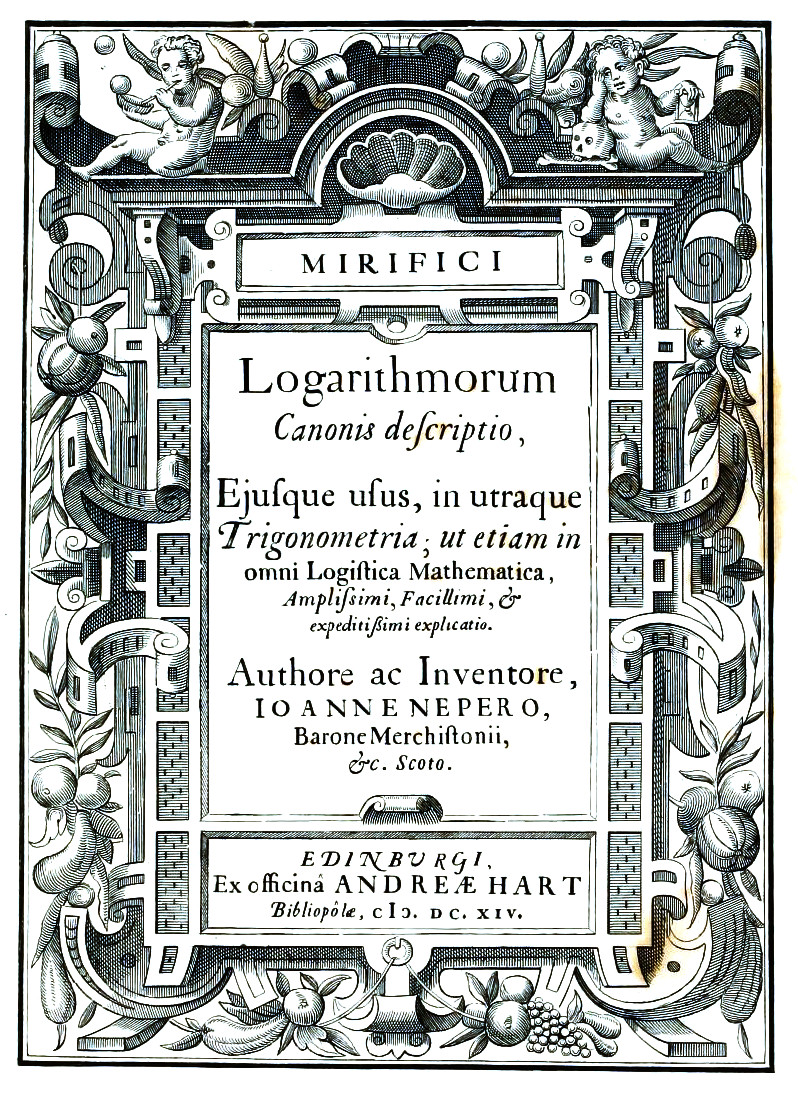
\includegraphics[width=1.75in]{Logarithms_book_Napier}
\end{minipage}
\hfil 
\begin{minipage}{0.7\textwidth}
    {\itshape
    Wonderful.

    The canonical description of logarithms 
    and its use in both trigonometry as well as in all mathematical logic.

    The most magnificent, quickest and most detailed explanation by the
    author and inventor 
    John Napier, Baron of Merchiston and other Scots.
    }
    % \vspace{0.5\onelineskip}
    \begin{itemize}[fullwidth]
        \item Logarithms were invented before \gap{calculators}.
        \item They were a \gap{device} to make math calculations easier.
        \item Astronomy, geodesy, trigonometry, spherical trignonometry, \dots
        \item $\approx$ 1600
    \end{itemize}
\end{minipage}
\hfil 

\begin{tcolorbox}[center,colback=white,width=5.5in]
    \gap{Logarithms} are a way of looking \gap{differently} 
    at \gap{exponential} expressions.
\end{tcolorbox}